\documentclass[acmsmall,screen,review,anonymous]{acmart}

% ============================================================
% Packages (see packages.sty)
% ============================================================
\usepackage{packages}
\ifPDFTeX\pdfdecimaldigits=5\fi
\microtypesetup{expansion=false}

% ============================================================
% Custom commands (see commands.sty)
% ============================================================
\usepackage{commands}
% Component reference: F258 Table II, physical page 11. PDF units are bp.
% Local definitions only: ACM document class, caption format and body remain.
\RequirePackage{colortbl}
\definecolor{F258Low}{rgb}{0.61412,0.85255,0.52313}
\definecolor{F258MidLow}{rgb}{0.79138,0.88196,0.72548}
\definecolor{F258MidHigh}{rgb}{0.95609,0.72275,0.72275}
\definecolor{F258High}{rgb}{0.91333,0.53333,0.53333}
\newcommand{\FTTableSetup}{%
  \fontencoding{T1}\fontfamily{ptm}\selectfont
  \fontsize{8.369bp}{10.54bp}\selectfont
  \setlength{\arrayrulewidth}{0.33432bp}%
  \setlength{\doublerulesep}{1.67412bp}%
  \setlength{\tabcolsep}{4bp}%
  \renewcommand{\arraystretch}{1.0}}
% Explicit adaptation: shade 1-F1 in quartiles, not counts or significance.
% Values exactly at a risk boundary enter the higher-risk bin.
\newcommand{\FTFScore}[1]{%
  \ifdim#1pt>0.75pt\cellcolor{F258Low}\else
  \ifdim#1pt>0.50pt\cellcolor{F258MidLow}\else
  \ifdim#1pt>0.25pt\cellcolor{F258MidHigh}\else
  \cellcolor{F258High}\fi\fi\fi#1}

\citestyle{acmnumeric}
\setcopyright{none}
\settopmatter{printacmref=false}
\acmDOI{}
\acmISBN{}
\acmConference[FSE 2027]{The ACM International Conference on the Foundations of Software Engineering}{July 12--16, 2027}{Shenzhen, China}
\acmYear{2027}

% ============================================================
% Document
% ============================================================
\begin{document}

\title[\toolname]{\toolname: Provenance-Guided Refinement of LLM-Generated Vulnerability Checkers}

\author{Anonymous Author(s)}

\begin{abstract}
Recent work shows that LLMs can synthesize static-analysis checkers from security patches, but a compilable checker is not necessarily a correct one.
A patch reveals what changed, not why the change is safe, so generated checkers often match only the surface edit and miss the deeper semantic condition.
Existing refinement loops feed back compilation errors and validation reports, yet these signals describe symptoms without explaining what the checker misunderstands about the code.

We observe that the analysis framework itself already computes the information needed to close this gap.
Control-flow graphs, symbolic values, memory regions and checker callbacks are available inside the analyzer but unused by current refinement strategies.
\toolname is a plug-in refinement layer that extracts patch-relevant analyzer evidence and assembles it with source context and validation feedback into a structured, provenance-labelled bundle.
An iterative editing loop refines the checker on both the vulnerable and fixed revisions, guarded by a retention gate that accepts warning recovery or false-positive reduction while preventing over-pruning.

We evaluate \toolname on 39 KNighter-derived CSA checkers from Linux kernel fixes.
With analyzer evidence, refinement reaches 23 warning-positive vulnerable revisions (vs.\ 15 for KNighter's loop) and raises version-level $F_1$ from $0.448$ to $0.575$.
Removing internal evidence yields nearly the same $F_1$ with fewer fixed-side reports.
Additional experiments cover three editor models on a 12-subject subset, a CodeQL query refinement, and controlled source-form variations.
A qualitative follow-up on all 11 non-tied comparisons shows how evidence helps repair checker recognition, and why the resulting warnings can still concern the wrong object, scope or path.

\end{abstract}
\ccsdesc[500]{Software and its engineering~Automated static analysis}
\ccsdesc[300]{Security and privacy~Systems security}
\keywords{static analysis, vulnerability checkers, large language models, patch-guided refinement}
\maketitle

% ============================================================
% Main body (FSE 2027: up to 18 pages of text and figures)
% ============================================================

\section{Introduction}\label{sec:intro}
Static analysis is a cornerstone of software security assurance for systems code.
Tools such as CodeQL~\cite{codeqlDocs} and Clang Static Analyzer (CSA)~\cite{clangsaDocs} detect vulnerabilities by checking source code against predefined rules without executing it~\cite{engler2001bugs,bessey2010coverity,calcagno2015infer,sadowski2015tricorder}.
The effectiveness of these tools depends on the quality of their vulnerability checkers, each of which must encode the semantic conditions that distinguish a real bug from safe code.
Writing such checkers by hand requires expertise in both the target codebase and the analysis framework, making manual authoring expensive and difficult to scale.

LLM-based patch-driven synthesis offers a promising alternative.
In this paradigm, a security patch serves as a compact before/after specification: the LLM consumes the patch and synthesizes a checker that should fire on the vulnerable revision but remain silent on the fixed revision.
KNighter~\cite{yang2025knighter}, a representative system, has demonstrated that this approach can produce compilable and executable CSA checkers from historical Linux kernel fixes.

However, the resulting checkers may be semantically inadequate.
A security patch is inherently underspecified: a one-line \texttt{goto}-target change may encode an ownership barrier, a widened cast may encode a range guard, and a moved \texttt{free} may encode a lifetime invariant.
A checker that captures only the syntactic shape of the edit can fire on both revisions or miss the vulnerable revision altogether.
Refinement can also remove a useful trigger while suppressing unwanted reports, a failure mode we call over-pruning.

Current refinement strategies, including KNighter's own iterative loop, use compilation and report feedback to guide further edits~\cite{yang2025knighter,madaan2023selfrefine,shinn2023reflexion}.
The checker, patch and reported path help the model reason about the failure.
Even with this context, however, a symptom such as “the vulnerable side is silent” may leave the implementation problem unclear.
A cleanup attribute may name a lowered callback that the checker never recognizes; a cast may hide the expression expected by a callback; or a state lookup may use a different region from the preceding update.

We observe that the analysis framework already exposes information useful for understanding these mismatches.
CSA provides compiler representations and observations of symbolic values, regions and checker callbacks.
CodeQL provides a different interface through its program database and queries~\cite{avgustinov2016ql,codeqlDocs}.
Exploiting this information requires selecting the relevant part of an analyzer's output, relating it to the patch and checker, and distinguishing it from ordinary reports or source text.

We present \toolname, an evidence-guided refinement framework for LLM-generated vulnerability checkers.
\toolname is designed as a plug-in post-generation layer, treating a generated checker as an artifact to be refined rather than regenerated.
First, rule-guided preflight selects patch-relevant evidence requirements.
Second, the collected facts, source context and validation feedback are normalized into a typed evidence bundle, with the origin and unavailable evidence recorded explicitly.
Third, the agent edits the checker and validates it on both revisions.
A retention gate keeps vulnerable-side warning recovery or fixed-side report reduction while rejecting the loss of an existing vulnerable-side warning.

We evaluate the workflow on all 39 selected generated-only CSA checkers from KNighter's artifacts.
Native refinement recovers eight initially silent vulnerable revisions, compared with six without internal evidence.
KNighter's report-driven policy makes no recovery edit on these silent starts.
The native and no-internal variants have nearly equal $F_1$, with 123 and 68 fixed-side reports, respectively.
Among the 15 initially noisy subjects, native refinement instead reduces fixed reports from KNighter's 69 to 44, largely through one subject.
These results led us to examine the actual edits and reports behind the differences.
An audit of all 11 non-tied comparisons, controlled perturbations of four mechanisms and repeated interventions at two checkpoints reveal useful recognition repairs alongside wrong-scope and infeasible-path warnings.
The evidence can help the checker recognize an operation without supplying all the conditions needed to report it correctly.

This paper makes the following contributions:
\begin{itemize}
  \item We present \toolname, a plug-in refinement layer that combines patch facts, source context, compiler representations and checker-execution observations in a typed, provenance-labelled evidence bundle.
  \item We provide a 39-checker comparison with KNighter's refinement loop and a no-internal variant, together with repeated decodes, model sensitivity and a separate CodeQL case.
  \item We analyze the code changes and diagnostic evidence behind the complete non-tie subset, explaining both useful local repairs and the semantic conditions they leave unresolved.
\end{itemize}


\section{Background}\label{sec:background}
\subsection{Static Vulnerability Checkers}

A vulnerability checker encodes a security-relevant condition within a static-analysis framework. Path-sensitive CSA checkers inspect callbacks, symbolic values, regions and state transitions; CodeQL queries operate over extracted program relations~\cite{clangsaDocs,avgustinov2016ql,codeqlDocs}. Industrial use demonstrates the value of static rules~\cite{engler2001bugs,bessey2010coverity,sadowski2015tricorder,calcagno2015infer}, but the framework does not make every custom checker's interpretation correct. Its rule must associate an operation with the right object, guards and lifetime. Report burden also affects use~\cite{johnson2013why,heckman2011alerts}; ranking and actionability prediction concern emitted reports~\cite{kremenek2002zranking,ruthruff2008actionable}, whereas refinement changes the code producing them.

\subsection{LLM-Based Patch-Driven Checker Generation}

Patches provide compact before/after evidence, building on semantic patching, clone-based vulnerability discovery and patch-derived datasets~\cite{padioleau2008coccinelle,jang2012redebug,kim2017vuddy,fan2020bigvul}. They are not complete specifications of all safe and unsafe uses. KNighter generates CSA checkers from Linux fixes and already refines them using compiler feedback, diagnostic/report-path context and validation on the original vulnerable/fixed pair~\cite{yang2025knighter}. Its no-report branch provides no report-driven edit. \toolname adds compiler/checker observations and attempts recovery from silence; it does not claim to introduce post-synthesis editing or paired validation.

\subsection{Analyzer-Internal Intermediate Results}

Backend intermediates expose how the analyzer represents the program, while checker-execution observations expose how a generated implementation uses that representation. Such facilities build on established graph, data-flow and interprocedural analyses~\cite{livshits2005finding,jovanovic2006pixy,arzt2014flowdroid,yamaguchi2014cpg}. They can clarify a mismatch without proving the reported vulnerability. We therefore distinguish backend-produced representations and observations, analyzer diagnostics, and source-derived context by actual provenance (Section~\ref{sec:evidence-roles}). A source window does not become an internal fact because an analyzer-labelled collector emits it; an internal fact does not become a correctness certificate because its raw origin is verified.


\section{Motivating Example}\label{sec:motivating}
This section traces one refinement instance end to end, using the KNighter-derived CSA checker for Linux commit \texttt{97cba232549b}, which repairs an off-by-one access in the AMD display driver~\cite{linuxCommit97cba232,yang2025knighter}.
The case is small enough to inspect manually yet exhibits the core problem.
The generated checker recognizes a look-ahead access but misses the relation between the loop bound and the array's capacity.

\textbf{The bug and its patch.}
The member \lstinline|dc->links| has declared capacity \lstinline|MAX_PIPES * 2|, abbreviated as $N$ in Figure~\ref{fig:motivating} (\cmark{1}).
The function \lstinline|get_host_router_total_dp_tunnel_bw| iterates over candidate links.
On a matching host-router branch, it reads both \lstinline|links[i]| and \lstinline|links[i + 1]| (M10--M11, \cmark{3}).
With the original condition $i<N$ (M5, \cmark{2}), the loop permits $i=N-1$, so the look-ahead can reach index $N$, outside the array.
The patch changes the bound to $i<N-1$ (M6, \cmark{4}), limiting the largest look-ahead index to $N-1$.
Other branch conditions determine whether the access occurs; the new loop bound prevents this final out-of-range access.

\begin{figure}[!htbp]
  \centering
  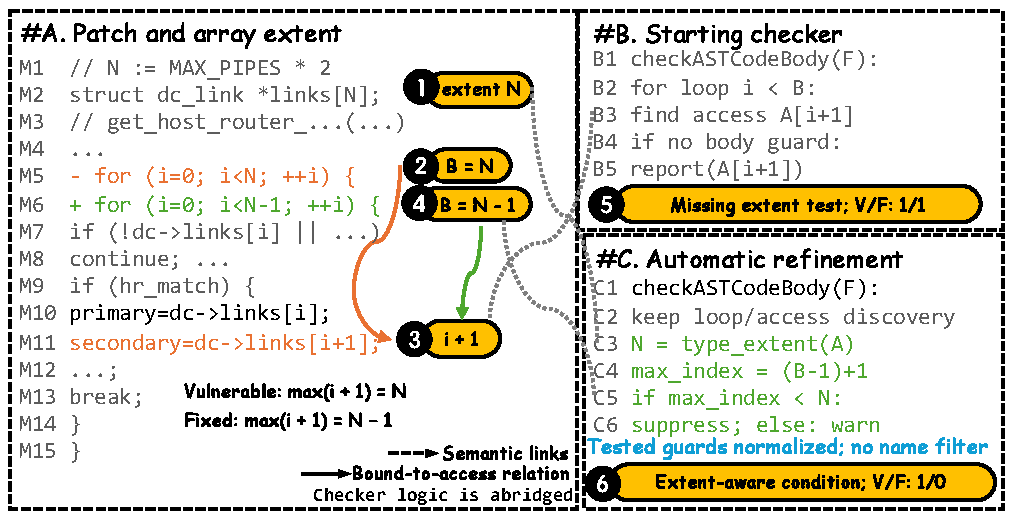
\includegraphics[width=0.70\textwidth]{figures/manual/motivating-example.pdf}
  \Description{A three-panel example. The left panel shows the array extent
  and the loop-bound patch. The upper-right panel shows the original
  look-ahead checker, which ignores the bound-to-capacity relation. The
  lower-right panel adds the maximum-index comparison while retaining the
  AST-based checker. Solid arrows relate loop bounds to the access; dashed arrows
  connect checker conditions to code.}
  \caption{\textbf{Capacity-aware look-ahead refinement.}
  Abridged code: $N$ denotes \lstinline|MAX_PIPES * 2| and
  \texttt{hr\_match} host-router equality. Independent vulnerable/fixed alerts
  change from \texttt{1/1} to \texttt{1/0}. This 14-response illustration used
  fixture feedback and differs from the one-response main-study checker.
  Orange/green arrows connect the bounds to the access; gray dotted links mark
  semantic correspondences.}
  \label{fig:motivating}
\end{figure}

\textbf{Why the baseline checker fails.}
The generated checker already recognizes an induction variable, a loop bound, and a look-ahead array subscript.
It reports an access when it does not recognize a protective condition in an enclosing \lstinline|if| (B1--B5, \cmark{5}).
That rule overlooks a guard carried by the loop condition itself.
The fixed program still contains \lstinline|links[i + 1]|, so the checker reports on both revisions despite the reduced loop bound.
Independent patch-related-object replay yields \texttt{1/1} alerts.
The checker has learned that a look-ahead access needs a guard, but not how the loop condition already supplies one.

\textbf{Evidence-guided refinement.}
\toolname starts from the same validation symptom and assembles the available patch, source and analyzer context.
This bundle has four provenance-labelled records: two internal Clang~18 CFG/call-graph records and two analyzer-output records.
The internal records anchor the loop and branch context to raw \texttt{debug.DumpCFG} and \texttt{debug.DumpCallGraph} output; patch and source context identify the bound change.

Both the starting and refined checkers use \lstinline|checkASTCodeBody|; the initial GLM-5.3-Flash edit adds a capacity-aware condition to the existing traversal.
The emitted checker reads the declared array extent from the AST type.
For the loop $i<B$, the maximum look-ahead index is $(B-1)+1=B$.
It suppresses the warning when that index is smaller than the known extent $N$ (C3--C6, \cmark{6}).
Thus the vulnerable $B=N$ remains reported, while the fixed $B=N-1$ becomes silent.
The condition uses type and index relations rather than the patched function name, a particular capacity, or adjacency of statements.
After two model calls, the candidate passes independent Linux replay at \texttt{1/0}.

\textbf{Checking the refinement.}
Further probes expose shortcomings in the candidate's fallback and inherited guard recognition.
Four automatic GPT-6-Luna-high quality continuations use 12 additional calls to repair these problems, giving 14 calls in total.
They receive the recorded fixture diagnostics; every scored checker edit is model-produced, and failed intermediate versions are retained.
The final checker still reports \texttt{1/0} on the Linux pair.
It passes 28 core fixtures, six boundary fixtures, 20 additional guard/bound fixtures, and 60 renamed/capacity-varied executions of those 20 forms: 58/58 unsafe and 56/56 safe executions overall.
AddressSanitizer also checks the labels of the latter 80 executions~\cite{serebryany2012asan}.

These tests cover name changes, unrelated statements, constant capacities and equivalent unit-step-loop/guard forms.
They informed the refinement, so they are a finite development suite rather than unseen-data confirmation or 114 independent bugs.
Arbitrary aliasing, dynamic extents and non-unit loop updates remain outside the tested forms.
The stronger illustration is kept separate from the 39-case experiment: its one-response G21 checker also reports \texttt{1/0} on the Linux pair but passes 74/114 of these fixtures.
Neither version isolates the contribution of internal records from the other supplied context.


\FloatBarrier
\section{Approach}\label{sec:approach}
\toolname is a post-synthesis refinement layer for LLM-generated vulnerability detectors.  Given a draft CSA checker or CodeQL query produced by an upstream generator, the patch that motivated the synthesis, and the corresponding source tree and validation scope, \toolname refines the detector to encode missing semantic predicates while retaining a vulnerable-side warning signal.

% \subsection{Overview}

\begin{figure}[!htbp]
  \centering
  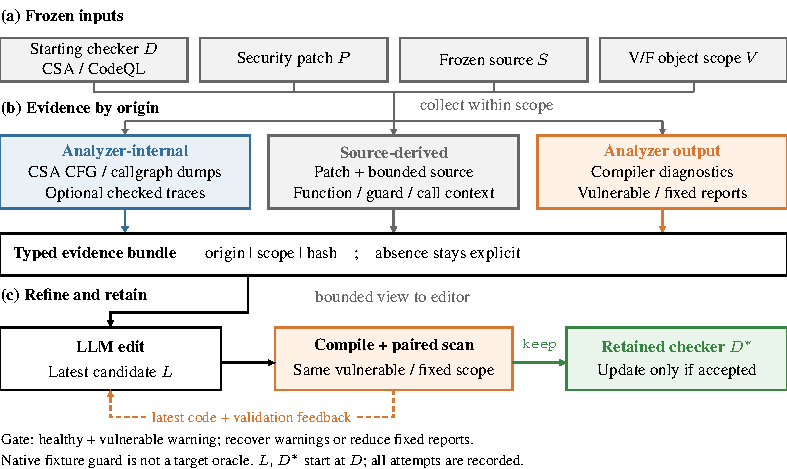
\includegraphics[width=\textwidth]{figures/fig-architecture-f258.pdf}
  \Description{Workflow from a generated checker and patch through evidence collection, a typed provenance-labelled bundle, checker editing, paired validation, and audit artifacts.}
  \caption{\textbf{\toolname architecture.}
  A generated detector, patch and bounded evidence feed the editor and paired retention rule. Native provenance is checked separately from collector names. Retention tracks version-warning presence, not target correctness; fixed silence is secondary. Inputs, rejected/retained candidates and raw validation records remain auditable.}
  \label{fig:approach-architecture}
\end{figure}

Figure~\ref{fig:approach-architecture} groups the workflow into three panels.
\textbf{(a)~Generator context.} The input is an existing detector, patch, source tree and validation scope, not a new generation task.
\textbf{(b)~Assembly and bundle.} Rule-guided preflight, source extraction, analyzer collection and validation feedback supply provenance-typed records and bounded views (Sections~\ref{sec:adaptive-selection}--\ref{sec:evidence-schema}).
\textbf{(c)~Paired-warning refinement.} The agent edits the latest attempted detector; normal paired outcomes update a separate best detector when they recover warning presence or reduce fixed reports while retaining it. Rejected attempts remain next-step input/feedback (Section~\ref{sec:refinement}).
\textbf{Audit artifacts.} The verifier checks raw-output/source-scope bindings, interfaces, provenance counts, selected code and paired logs. Original prompts, replies and all attempts persist; an LLM explanation is not an origin certificate.

\begin{algorithm}[t]
\footnotesize
\caption{Paired-Warning Evidence-Guided Refinement}
\label{alg:evidence-guided-refinement}
\begin{algorithmic}[1]
\Require detector $D$, patch $P$, source $S$, scope $V$, backends $A$, budget $K$
\Ensure refined detector $D^*$ and audit report
\State $R_0 \gets \Call{Validate}{D,P,V}$
\State $E_p,E_s \gets \Call{Preflight}{P},\ \Call{ExtractSource}{P,S,D}$
\State $E_a \gets \bigcup_{a\in A}\Call{CollectNative}{a,D,P,S}$ \quad $E_v \gets \Call{Feedback}{R_0}$
\State $B \gets \Call{NormalizeMerge}{E_p,E_s,E_a,E_v}$
\State \textbf{if} $\Call{PDS}{D,P,V}$ \textbf{then return} $\Call{Audit}{D,B}$
\State $D^* \gets D$ \quad $L \gets D$ \quad $T \gets \Call{InitialStopState}{}$
\For{$i=1$ to $K$}
  \State $V_i \gets \Call{BoundedView}{B}$ \quad $C_i \gets \Call{AgentEdit}{L,P,V_i}$
  \State $R_i \gets \Call{ValidateIfCompilable}{C_i,P,V}$
  \State \textbf{if} $\Call{Accept}{C_i,D^*}$ \textbf{then} $D^* \gets C_i$ \Comment{Equation~\ref{eq:accept}}
  \State $L \gets C_i$ \quad $E_i \gets \Call{Feedback}{R_i}$
  \State $B \gets \Call{Merge}{B,E_i}$
  \State $T \gets \Call{UpdateStopState}{T,R_i,D^*}$
  \State \textbf{if} $\Call{Stop}{T,K}$ \textbf{then break}
\EndFor
\State \Return $\Call{Audit}{D^*,B}$
\end{algorithmic}
\end{algorithm}

\subsection{Evidence Selection and Exposure}
\label{sec:adaptive-selection}

The central design choice in evidence assembly~(Figure~\ref{fig:approach-architecture}b) is \emph{what to collect and expose}.  Analyzer outputs can be large and heterogeneous; passing them wholesale to the editor obscures patch-relevant relations.  The preflight planner represents candidate requirements by role and priority, while source/function scope and bounded views limit what the editor sees.  In the strict CSA comparison, collection is precomputed and the visible view is frozen, so its result does not measure demand-driven routing.

\textbf{Rule-guided preflight and role requests.}
The implementation has no separately trained or prompted patch-mechanism classifier.  \texttt{PatchFacts\allowbreak Extractor} parses the patch and metadata for affected functions, added guards, risky calls, and type widenings.  \texttt{Evidence\allowbreak Planner} takes a primary pattern from analysis metadata when available or infers it from those facts, then assigns fixed priorities to requirements: patch anchoring is 100, lifetime/state requirements for double-free or use-after-free are 92/89, and a guard for null or bounds cases is 90.  It sorts by descending priority with evidence type as a tie-breaker and retains at most eight planned requirements in the default configuration.  Table~\ref{tab:evidence-routing} summarizes mechanism-to-role examples; it is not a classifier confusion matrix or a promise that every role is analyzer-internal.  The normalizer does not learn or re-rank facts.  In the general workflow the editor may request evidence types, with duplicate and request-count limits.
For the audited CSA comparison, static records are precomputed and additional requests disabled. The selected v43 implementation resolves compiler references into at most four function-local CFG witness cards, selected with patch/report scope; graph dominance is not path feasibility. It contrasts compiler/checker state associations and helper spelling with the detector, appending available execution observations. No-internal receives neither native witness nor dynamic views, but keeps patch, frozen source and ordinary feedback. This bounded deterministic exposure is not a classifier or a measured optimal routing policy.

\begin{table}[!htbp]
\centering
\caption{Rule-guided evidence requirements by patch mechanism (representative); names are persisted record types, not gold labels or measured classifier outputs.}
\label{tab:evidence-routing}
\begingroup\FTTableSetup
\begin{tabular}{p{0.30\columnwidth}|p{0.42\columnwidth}|p{0.18\columnwidth}}
\hline\hline
Patch mechanism & Possible record types & Backend \\
\hline
Cleanup edge / double free & \texttt{allocation\_lifecycle}, \texttt{state\_transition}, \texttt{path\_guard} & CSA \\
Bounds widening / overflow & \texttt{semantic\_slice}, \texttt{dataflow\_candidate}, \texttt{state\_transition} & CSA/CodeQL \\
Initialization / null deref & \texttt{state\_transition}, \texttt{path\_guard} & CSA \\
Use-after-free / escape & \texttt{allocation\_lifecycle}, \texttt{call\_chain} & CSA/CodeQL \\
API misuse / missing check & \texttt{semantic\_slice}, \texttt{call\_chain} & CodeQL \\
\hline\hline
\end{tabular}
\endgroup
\end{table}

\subsection{Evidence Sources and Roles}
\label{sec:evidence-roles}

Four collectors execute in sequence; Figure~\ref{fig:approach-architecture}b groups views by origin rather than execution order. \textbf{Patch preflight} locates changed files/hunks and mechanism context. \textbf{Source extraction} resolves function, guard, call, state and build context in bounded views, without repository-scale dumps.

\textbf{Analyzer evidence} is classified by its actual origin, not by the collector's name.  We call a record \emph{analyzer-internal} only if its payload is derived from a backend-produced intermediate representation, identifies the interface and raw output, and is bound to a source revision, file, and function.  In the measured CSA cohort the interface is Clang 18's \texttt{debug.DumpCFG} and \texttt{debug.DumpCallGraph}; the persisted UTF-8 dump is parsed into schema \texttt{semweaver.csa\_cfg\_snapshot.v1}, with a raw-output SHA-256 and source-scope binding.  These dumps provide CFG branches and value bindings and call edges.  They do \emph{not} themselves prove a path-feasible lifetime or ownership transition.  Analyzer diagnostics and alert counts are \emph{analyzer output}, not internal state.  Patch diffs, source windows, and compile-database-assisted source extraction are \emph{source-derived} fallbacks even when a CSA or CodeQL collector emits them.  A live CodeQL database query could meet the internal-evidence definition if its query, database revision, and tuples were retained; we do not attribute source-window-derived CodeQL facts to that category.

The selected implementation also observes instrumented CSA callbacks, abstract values/regions and checker-state associations. Raw JSONL uses \texttt{semweaver.checker\_trace.v2}; bounded feedback uses \texttt{semweaver.trace\_feedback.v1}. This is not concrete execution or exhaustive symbolic-state proof. Original/instrumented scans must preserve diagnostics on both revisions; caps, live fixtures and input hashes distinguish valid absence from broken instrumentation.

Extraction must handle verbose, backend-specific intermediates and instrumentation that may shadow identifiers, exceed caps or see no eligible callback. Revision, architecture, scope and parity checks retain missing observations as unavailable. Table~\ref{tab:origin-types} partitions 193 records across all 39 subjects. Its 81 native records comprise 45 guards, 27 state-transition and 9 allocation-lifecycle records; all 61 source-derived records are patch diffs, not source-window fallbacks. Attached context is not itself native. Dynamic availability is per-attempt (RQ3).

\begin{table}[!htbp]
\centering
\caption{Evidence primitives and provenance in the audited 39-case CSA cohort. One record may contain several CFG primitives; counts are by record origin, not primitive.}
\label{tab:origin-types}
\begingroup\FTTableSetup
\begin{tabular}{p{0.27\columnwidth}|p{0.53\columnwidth}|c}
\hline\hline
Origin & What the persisted record contains & Records \\
\hline
Analyzer-internal & Clang CFG guards, value bindings and call edges; raw-output and scope binding & 81 \\
Analyzer output & CSA diagnostics and paired validation reports; no internal state & 51 \\
Source-derived & Patch-diff records here; other interfaces may emit source-window fallbacks & 61 \\
\hline\hline
\end{tabular}
\endgroup
\end{table}

\textbf{Validation feedback} records compilation, execution health and paired warnings: symptoms to diagnose, not semantic ground truth.

% \smallskip
\begingroup\emergencystretch=2em
The seven persisted types are \texttt{patch\_fact} (changed statements), \texttt{semantic\_slice} (bounded statements, guards, API terms and symbols), \texttt{dataflow\_candidate} (possible propagation), \texttt{call\_chain} (call context), \texttt{path\_guard} (control), \texttt{allocation\_lifecycle} (resources), and \texttt{state\_transition} (abstract state). ``Barrier,'' ``type filter,'' and ``API usage'' interpret record content; they are neither extra types nor proven path feasibility.
\par\endgroup

When a selected role yields no evidence, the bundle retains an explicit missing-evidence marker rather than treating the absence silently, so the refinement agent knows what was requested but unavailable.

\subsection{Evidence Bundle Schema}
\label{sec:evidence-schema}

The normalizer merges all collected facts into the \texttt{EvidenceBundle} shown in Figure~\ref{fig:approach-architecture}b.  Each fact becomes an \texttt{EvidenceRecord} carrying a type, the contributing analyzer, scope, source location, payload, provenance, and an optional \texttt{EvidenceSlice} (the compact semantic content consumed by the agent).  The schema separates program facts from analysis rules in the spirit of relational analyzer frameworks~\cite{avgustinov2016ql,jordan2016souffle,bravenboer2009doop}, but uses a smaller role vocabulary tailored to checker refinement.  Formally:
\begin{equation}
\begin{aligned}
B &= \mathrm{Norm}(E_p \cup E_s \cup E_a \cup E_v),\\
E_a &= E_{\mathrm{CSA}} \cup E_{\mathrm{CodeQL}},\\
r &\in B.records = \langle type, analyzer, scope,\\
&\quad location, payload, provenance, slice\rangle.
\end{aligned}
\label{eq:evidence-bundle}
\end{equation}
Here $E_p$ contains patch facts, $E_s$ bounded source slices, $E_a$ analyzer-internal representations \emph{or} outputs filtered by selected roles (Section~\ref{sec:adaptive-selection}), and $E_v$ validation outcomes. Each record's provenance has one of three origins: \texttt{analyzer\_\allowbreak internal}, \texttt{analyzer\_\allowbreak output}, or \texttt{source\_\allowbreak derived}. The normalizer deduplicates records and marks missing evidence; origin is neither a confidence score nor a proof of semantic correctness.

The type-to-backend mapping reflects available interfaces: CSA CFG/call-graph dumps inform guard, state, and call-chain records; CodeQL queries can support flow and relation records when a live database is available.  These are record types, not seven distinct backend analyses.  Cross-function call edges provide context, but the present CSA dump does not establish an interprocedural path or ownership proof.  Provenance remains visible when a type is populated only by a fallback.

The bundle is bounded by design: scope and selected views limit raw dumps. The matched pipeline contrast and repeats remain subject to selection history, stochastic draws and bundled native components; they do not isolate each representation's causal effect.

\subsection{Paired-Warning Refinement}
\label{sec:refinement}

The refinement loop (Figure~\ref{fig:approach-architecture}c) receives the current detector, patch, baseline validation notes, and a bounded role-specific evidence view.  The interface supports requesting further roles from the persisted bundle, but the provenance-audited matched condition freezes the visible view before the edit and disables additional agent requests.  Thus its measured effect is a contrast between preselected native-evidence and no-internal views, not a test of dynamic evidence retrieval.  This keeps the prompt bounded and the two conditions auditable.

The agent's tool-mediated loop draws on recent LLM agent and self-refinement architectures but constrains actions to attached evidence, detector edits, and validation commands~\cite{madaan2023selfrefine,shinn2023reflexion,yao2023react,schick2023toolformer}.  Where evidence requests are enabled, they replay attached records rather than launch open-ended repository exploration; the request count is capped and unused or missing evidence is logged.  In the matched condition, request count is zero by protocol.

\textbf{Model versus deterministic components.}  LLMs may produce patch-analysis metadata and the editor's checker edit; when enabled, the editor also chooses which evidence types to request.  The preflight requirement rules, raw-output hashing and scope binding, record normalization, checker compilation, paired replay, and acceptance are programmatic.  The LLM does not create a backend dump, set a provenance origin, or decide PDS.  The audit retains the exact starting checker, prompt and response, visible roles, raw evidence, candidate source, and validation decision.  This boundary prevents an LLM explanation from being counted as analyzer-produced evidence.
The editor prompt supplies the current and starting checker paths, patch path, bounded source/evidence view, baseline vulnerable/fixed symptom, backend identity, and edit/validation rules.  It asks for an in-place checker edit that models the mechanism rather than matching patch spellings, forbids suppressing the vulnerable trigger, and requires compilation before paired acceptance.  Compiler-repair prompts receive the actual build diagnostics; all available English templates and rendered exchanges are named in the artifact manifest, with absent historical raw exchanges explicitly marked rather than reconstructed.

\textbf{Retention gate.} Changed candidates must compile and receive normal paired execution. Equation~\ref{eq:accept} retains warning recovery from silence, or lower fixed reports with a nonzero vulnerable signal. PDS is stronger but not mandatory. The native-only controlled-fixture guard preserves required existing hits; it is not a target oracle. Silencing an existing vulnerable signal is rejected. A comparative disadvantage against control may instead reflect failure to recover from initial silence or a smaller improvement.

\textbf{Feedback loop.} The next permitted reply edits the latest attempt using its build or paired feedback, while the best retained detector is separate. Rejected and invalid edits remain visible. Positive/fixed-silent saturation, three valid non-improving validations, three consecutive invalid attempts or the reply cap stops the case (Algorithm~\ref{alg:evidence-guided-refinement}). Execution interruptions are unscored and repaired without resampling consumed prefixes. The 15-case report-refinement view uses the same full-cohort outputs; it is not a separate per-case-budget experiment.

\textbf{Backend extension surface.}
An adapter must provide registration, evidence/provenance mapping, dependencies, execution/result decoding, and paired validation. Shared modules still contain backend branches. Four enumerated CodeQL-specific modules occupy 2,438 physical lines, including comments and generation code: an existing footprint, not code to rewrite for each backend. With a usable analyzer and patch pair, we estimate that a familiar developer using Codex can complete basic adaptation within an afternoon by reusing these interfaces. This is a planning estimate, not measured labor or a scalability result. New native-evidence semantics and broad validation require separate work. The artifact lists prerequisites and tasks. A new bug mechanism needs a role mapping and safe/unsafe fixtures, and a new extractor only for unavailable relations.

% \subsection{Outputs}

% Each run writes the refined detector, normalized evidence bundle, preflight plan, validation feedback, refinement manifest, analyzer result records, and final report, so a refinement instance can be audited or resumed without reconstructing experiment state.


\FloatBarrier
\section{Evaluation}\label{sec:evaluation}
We evaluate whether analyzer evidence helps \toolname recover vulnerable-side warnings and reduce fixed-side reports.
The evaluation focuses on patch-local and patch-related-file behavior rather than whole-kernel bug discovery.

\subsection{Research Questions}

\noindent\textbf{RQ1: KNighter-derived checkers.} How does \toolname compare with KNighter's refinement loop on vulnerable-version warning coverage, fixed-side report burden and paired discrimination?

\noindent\textbf{RQ2: Cross-backend feasibility and cost.} Can the refinement layer operate on an archived CodeQL query associated with an earlier automatic generation run, and what integration and execution costs are observable?

\noindent\textbf{RQ3: Evidence contribution.} How do the native and no-internal variants differ, and what do their edits and reported gains establish?

\noindent\textbf{RQ4: Model sensitivity.} How does the workflow perform with three editor configurations on the same subset under common reply and output ceilings?

\subsection{Experimental Setup}

\subhead{Subjects and benchmarks.}
We organize the evaluation into four experiments (E1--E4).
E1 uses KNighter-derived Linux CSA checkers under patch-related object validation.
From 286 artifact records on 60 commits, 241 records on 39 commits lack an upstream refinement-status row.
We select one nonempty repaired-source artifact per commit by upstream TP, then TN, then the lowest checker index.
This fixed, non-random rule selects the inputs; independent paired replay supplies their starting outcomes.
All 39 enter KNighter refinement and both \toolname variants, including cases that remain noisy or fail to improve.
Initially, 15 checkers warn on both revisions and 24 are silent on both.
Their zero starting PDS is the study's entry state.

The 15 initially noisy checkers also form a complete report-refinement stratum.
Its results reuse the full-cohort outputs.
For the 24 silent starts, KNighter's no-report branch compiles without a model edit, whereas \toolname attempts recovery.
We report these branches as the systems execute them.

The selected implementation is v43, chosen after comparing two configurations on six experimental subjects.
Compatible executions on those subjects are reused in E1; the configuration-selection cases overlap the evaluation.
The artifact retains those trials and their reuse checks.
G04 uses its architecture-correct ARM64 scope and evidence after repair of an earlier wrong-object scan.

E2 uses an archived CodeQL input associated with an earlier automatic generation run, independently of KNighter, for ImageMagick (CVE-2017-12877, \texttt{coders/\allowbreak mat.c}).
All three refinement decodes start from this same query.
We report it separately from CSA.
Earlier 20-row results from mixed and manual inputs are excluded.
E3 compares native and no-internal on all 39 main pairs and repeats a 12-subject subset; E4 uses the same 12 subjects, native only, with three decodes per model (Figure~\ref{fig:study-design}).

Subset membership follows the initial scan status.
We sort SHA-256 hashes of a fixed artifact-recorded salt plus case ID within the original 14 noisy and 25 silent cases, then take the first 4 and 8.
A later scan repair corrects G08 from $0/0$ to $2/2$, leaving the same membership with 5 noisy and 7 silent subjects.
The selection uses no refinement outcomes or vulnerability-class stratification; it contains no bounds cases.

\begin{figure}[!htbp]
\centering
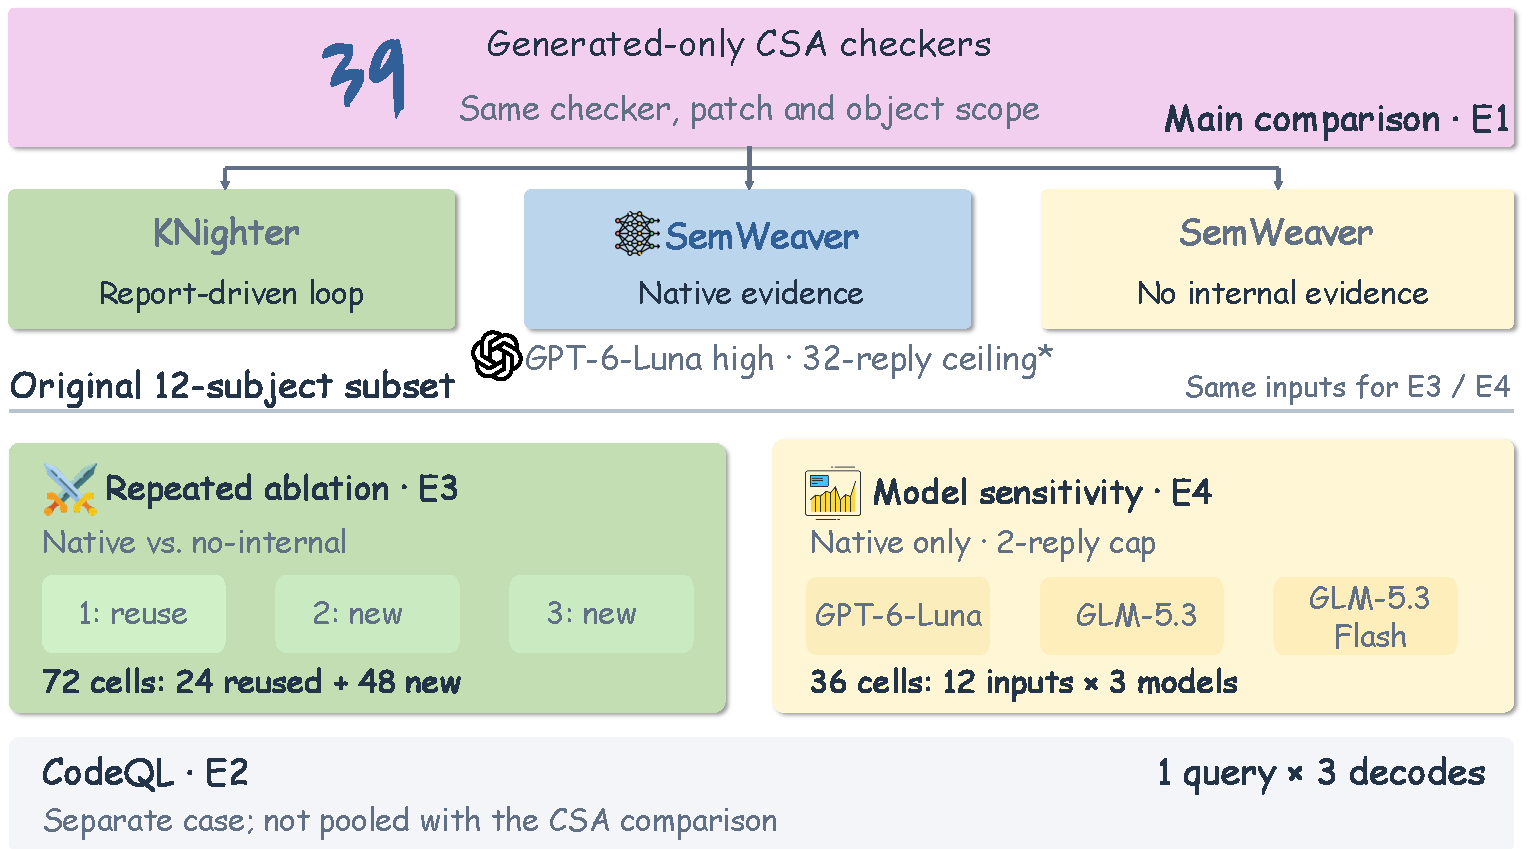
\includegraphics[width=0.70\textwidth]{figures/manual/study-design.pdf}
\Description{All 39 CSA checkers enter three main comparison arms. E3 and E4 use the same original 12-subject subset. E3 reuses 24 first-decode condition cells and adds 48. The drawing shows E4's first 36 native-only cells; two further decodes add 72, for 108 trial records. The CodeQL case is separate.}
\caption{\textbf{Experimental design and reuse.} E3's first decode reuses E1. The E4 panel depicts its first decode (36 cells); two further decodes add 72 cells, for 108 records on the same 12 inputs. Cells are not independent bugs. $^*$Audited natural-stop reuses retain original caps; shared ceilings do not imply equal realized effort.}
\label{fig:study-design}
\end{figure}

\subhead{Baselines and variants.}
We hold the generated detector fixed so that the comparison follows edits to the same checker rather than a fresh generation draw.
E1 native, no-internal and KNighter use the same requested GPT-6-Luna-high editor and a 32-reply ceiling.
KNighter retains its report-driven algorithm with five reports and two outer attempts, and its emitted checkers receive independent scans.
The 24 no-report branches consume no reply.
Two natural one-response No-FP stops are audited reuses that retain their original eight-reply ceiling; both terminate before either ceiling.
We report actual replies and warning counts alongside the common maximum.

Within \toolname, no-internal removes native compiler and checker-execution views while keeping the checker, patch, frozen source, build and paired-scan feedback, and stopping rule.
Native receives the bounded CFG witness and mismatch views and available dynamic observations.
E3 repeats the original 12 subjects at 32 replies and 16,384 output tokens per call.
E4 uses GPT-6-Luna high, GLM-5.3 high and GLM-5.3-Flash high, with three decodes per model, 2 replies per decode and 65,536 output tokens per call.
Actual GLM effort fields are retained.
Earlier default-effort, smaller-output and outside-subset histories are kept separate.
E4 has no no-internal arm across models.

\subhead{Experimental procedure.}
For each sample, we collect evidence, refine the detector and validate it on both revisions.
Each permitted reply counts as an attempt.
Compilable changed candidates receive independent paired replay and are retained under Equation~\ref{eq:accept}.
The next call receives the latest attempted code and feedback; the best retained detector is stored separately.
The loop stops when a vulnerable warning and fixed-side silence are achieved, after three valid validations without improvement, after three consecutive invalid model attempts, or at the reply cap.

We preserve failed attempts and consumed prefixes when repairing execution problems.
Thinking-only replies consume budget.
For one GLM reply containing an explicit action and three edits but no explanatory summary, network-disabled replay supplied an empty summary and reproduced the model-specified code with no new call.
Healthy zero-callback probes use static evidence.
Compilation failures, format failures, unavailable observations, provider interruptions and invalid scans remain distinct; no manual checker completion enters the scored results.

\subhead{Environment.}
CSA uses Clang/LLVM 18.1.3 and Python 3.12.3.
CodeQL uses version 2.26.4, \texttt{codeql/cpp-all} 8.0.3 and no-build databases.
Each Linux subject uses its patch commit and parent, \texttt{allyesconfig}, architecture-correct objects, and the same scope for starting, baseline and refined checkers.
Manifests record code, evidence and raw paired outputs.
The recorded model labels and high-effort requests identify the tested services.
Both Responses adapters omit the configured temperature field, and no fixed seed is used.

\subhead{Use of generative AI in the study.}
The editor models generated the checker and query edits evaluated in this study.
Codex assisted with the development of experimental tools.

\subsection{Metrics}

We report vulnerable-version warning presence and fixed-side report burden.
Let $n_v(D)$ and $n_f(D)$ count warnings in the same patch-related object scope on the vulnerable and fixed revisions.
The stronger outcome, \emph{patch-discriminating success} (PDS), requires a vulnerable-side warning and fixed-side silence:
\begin{equation}
\begin{aligned}
H_v(D,P,V)&=\mathbb{1}[\mathrm{alerts}(D,V_{\mathrm{vuln}},P)>0],\\
S_f(D,P,V)&=\mathbb{1}[\mathrm{alerts}(D,V_{\mathrm{fix}},P)=0],\\
\mathrm{PDS}(D,P,V)&=H_v(D,P,V)\land S_f(D,P,V).
\end{aligned}
\label{eq:pds}
\end{equation}
We distinguish two useful improvements.
\emph{Warning recovery} makes an initially silent vulnerable revision warning-positive, possibly with fixed-side noise.
\emph{Report reduction} lowers fixed-side reports while preserving vulnerable-side warning presence.
A detector that loses an existing vulnerable warning is rejected.
A comparative disadvantage means that another arm retains a better result, which may still be an improvement over the starting checker.

For retained detector $D^*$ and normally paired-executed candidate $C$, the improvement rule is:
\begin{equation}
\begin{aligned}
\mathrm{Accept}(C,D^*)={}&\mathrm{AnalyzerOK}(C)\land H_v(C)\\
&\land\bigl(\neg H_v(D^*)\lor n_f(C)<n_f(D^*)\bigr)\land Q(C).
\end{aligned}
\label{eq:accept}
\end{equation}
The editor requires a changed artifact before paired assessment.
$Q$ preserves required hits on controlled array fixtures in native and is identically true for no-internal.
This native-only guard records zero rejections in E1/E3.

For precision, recall and $F_1=2TP/(2TP+FP+FN)$, each vulnerable revision is a positive and its fixed revision a negative, classified by warning presence.
These metrics cover 78 patch-version decisions.
Fixed-side report counts measure inspection burden.
Neither measure adjudicates individual bug sites: G08, for example, warns on allocation failure rather than the registration-failure leak repaired by its patch.
The qualitative follow-up in Section~\ref{sec:target-results} examines target association separately; failed scans remain unscored.




\FloatBarrier
\section{Results}\label{sec:results}
\subsection{RQ1: Generated CSA Checkers}

Table~\ref{tab:all39-system} reports all 39 subjects and the preexisting 15-case noisy stratum. Zero starting PDS is an entry condition, not KNighter's refinement result. Every portfolio retains the 15 initially warning-positive vulnerable revisions. Among the 24 initially silent subjects, native recovers 8, no-internal 6, and KNighter 0 under its actual no-report policy. These are warning signals, not verified target-recall counts.

\begin{table}[!htbp]
\centering
\caption{CSA comparison: (a) all 39 subjects; (b) the complete preexisting 15-case fixed-noisy stratum, reusing the same outputs. TP/FP/FN are version-warning decisions; fixed reports measure burden and replies count received responses. Color shades $1-F_1$ at .25/.50/.75, not significance.}
\label{tab:all39-system}
\label{tab:matched14}
\begingroup\FTTableSetup
\begin{tabular}{l|cccc|c|cc}
\multicolumn{8}{l}{(a) Full cohort: 39 subjects}\\
\hline\hline
\multirow{2}{*}{Condition}&\multicolumn{4}{c|}{Version outcomes}&
\multirow{2}{*}{$F_1$}&\multicolumn{2}{c}{Burden / effort}\\
\cline{2-5}\cline{7-8}
&PDS&TP&FP&FN&&Fixed reports&Replies\\\hline
Unmodified &0&15&15&24&\FTFScore{.435}&73&0\\\hline
KNighter loop &2&15&13&24&\FTFScore{.448}&69&179\\\hline
\toolname, native &5&23&18&16&\FTFScore{.5750}&123&150\\\hline
\toolname, no internal &8&21&13&18&\FTFScore{.5753}&68&133\\
\hline\hline
\end{tabular}
\par\smallskip
\begin{tabular}{l|c|c|c}
\multicolumn{4}{l}{(b) Noisy 15: all methods retain TP=15, PDS=2 and $F_1=.6977$}\\
\hline\hline
& KNighter loop & Native & No internal\\\hline
Fixed reports &69&44&68\\
\hline\hline
\end{tabular}
\endgroup
\end{table}

Warning coverage and report burden move in different directions: native's 123 fixed reports exceed no-internal's 68 and KNighter's 69; its precision is $0.561$ versus $0.618$ for no-internal. The nearly tied $F_1$ summarizes different coverage/noise portfolios and does not establish native superiority. G12 contributes 73 distinct fixed-side warning locations, not duplicates; its broader matching yields 74 vulnerable and 73 fixed reports. This unfavorable tradeoff remains in the aggregate.

In the complete 15-case fixed-noisy stratum (Table~\ref{tab:matched14}b), native reduces reports by 25 (36.2\%) against KNighter and 24 (35.3\%) against control. The effect is concentrated in G24's $27\rightarrow2$ fixed reports; other small differences offset one another. Identical binary fixed positivity and $F_1$ thus coexist with different report burdens. The follow-up finds G24's retained reports outside the target lifecycle (Section~\ref{sec:target-results}); the lower count is therefore not evidence of target-preserving suppression.

\subsection{RQ2: Cross-Backend Feasibility}

A separate archived automatic ImageMagick CodeQL query starts at $0/0$ vulnerable/fixed rows. Table~\ref{tab:codeql-decoding} includes two $8/0$ recoveries and the third decode's $22/22$ outcome. The successful edit corrects relative-path matching while keeping exact file/function/local-variable filters. This demonstrates patch-local operation on a second format, not broad backend transfer or native-evidence causality. A second query already starts at $2/0$ and is not counted as a gain. KNighter is not a CodeQL baseline.

\begin{table}[!htbp]
\centering
\caption{Three automatic CodeQL decodes of one query. Counts are vulnerable/fixed output rows; time is recorded agent-round duration, excluding separate paired replay.}
\label{tab:codeql-decoding}
\begingroup\FTTableSetup
\begin{tabular}{c|c|crr}
\hline\hline
Decode & V/F rows & Replies & Tokens & Agent time (s)\\\hline
1 &8/0&1&15,122&87.87\\
2 &8/0&1&14,345&42.74\\
3 &22/22&8&110,282&516.77\\
\hline\hline
\end{tabular}\endgroup
\end{table}

\textbf{Second-backend costs.} Table~\ref{tab:codeql-decoding} reports the original model runs. Three warm paired replays per query preserve $0/0$ and $8/0$. Median query-plus-decode time is 12.57\,s initially and 36.51\,s after refinement with two threads; peak process RSS is 976/1,078\,MiB. Database-creation log intervals span 31/30\,s, excluding unlogged startup. Developer labor is unmeasured. These one-case existing-environment observations are neither a speedup, cold-install benchmark nor whole-project scalability estimate.

\subsection{RQ3: Internal-Evidence Sensitivity}

Table~\ref{tab:origin-types} reports initial record provenance; Section~\ref{sec:evidence-roles} defines native types and source-derived context. Dynamic availability has a separate denominator: 103 of 150 unique native-chain attempts have usable hash-bound observations; 11 are unavailable due to candidate compilation, 18 unsupported context, 13 zero scoped callbacks, 1 reproduced candidate crash and 4 capped optional observations. None establishes safety from absence.

Across 39 subjects, native has six comparative benefits, five disadvantages and 28 ties/other outcomes. The associated edits expose concrete differences in checker behavior: cleanup-wrapper recognition in G19, nested dereference/binding recovery in G25, and null/region/frame handling in G24. G19 adds \texttt{\_\_free\_kfree} to a cleanup predicate, yielding $15/0$ versus control's $0/0$; 15 reports are not 15 bugs. Conversely, control recovers symbolic-region handling in G23 and persistent-field release recognition in G38 without native records. G12 drops CPU-role restrictions, explaining its broad matching and noise. These code observations distinguish repairs from broader matching; a record's presence or an LLM explanation alone does not prove edit causality.

\begin{figure}[!htbp]
\centering
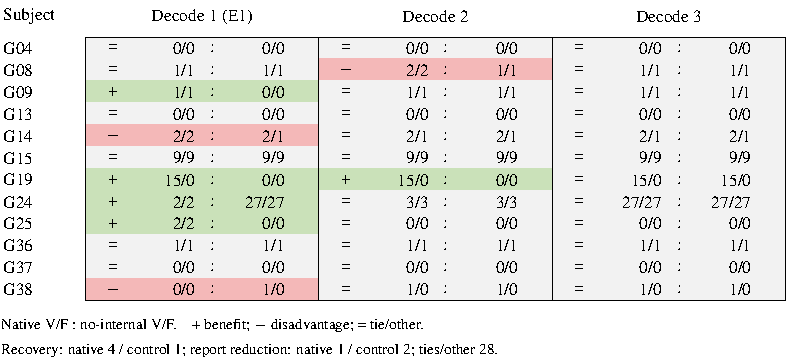
\includegraphics[width=378bp]{figures/fig-e3-repeats.pdf}
\Description{A twelve-subject by three-decode matrix of native and no-internal vulnerable/fixed warning counts, highlighting comparative benefits, disadvantages and ties.}
\caption{E3: all 36 paired decodes on 12 subjects; cells compare native and no-internal V/F counts. Decode 1 reuses E1; the remaining decodes add 48 condition cells. Color and sign encode the comparative direction.}
\label{fig:repeats}
\end{figure}

Figure~\ref{fig:repeats} shows five subjects tying in all three decodes and seven with mixed directions; none benefits comparatively in all three. G19's native $15/0$ recurs, but control catches up in its third decode. G24's main reduction does not repeat. G14's $3/3\rightarrow2/2$ improves its own start but trails control's $2/1$; later decodes tie. In the main comparison, G05/G23/G38 retain initially $0/0$ in native while control recovers warnings, so their disadvantage is not loss of an initial signal. Repeated subjects, selection/reuse and native-only gating limit stronger attribution. Realized call differences under a shared stopping rule are outcomes/mediators, not independently assigned confounds.

\subsection{RQ4: Model Configuration Sensitivity}

Table~\ref{tab:models39} uses the original 12 subjects, native only, one decode per model, 2-reply and 65,536-output ceilings with requested high effort. All configurations retain the five initial vulnerable warning signals and recover additional versions. Flash has the strongest observed outcome here, but one decode on this subset does not establish general ranking or variance-controlled model robustness.

\begin{table}[!htbp]
\centering
\caption{Limited-budget native sensitivity: 12 subjects per model, not full-39 robustness. Computation differs despite common reply/output ceilings. $F_1$ shading follows Table~\ref{tab:all39-system}.}
\label{tab:models39}
\begingroup\FTTableSetup
\begin{tabular}{l|ccc|c|cc}
\hline\hline
Editor & TP & FP & PDS & $F_1$ & Fixed reports & Replies\\
\hline
Unmodified &5&5&0&\FTFScore{.455}&42&0\\\hline
GPT-6-Luna high &7&6&1&\FTFScore{.560}&40&24\\\hline
GLM-5.3 high &7&5&2&\FTFScore{.583}&16&23\\\hline
GLM-5.3-Flash high &9&5&4&\FTFScore{.692}&11&21\\
\hline\hline
\end{tabular}
\endgroup
\end{table}

Received replies total 24/23/21 respectively. Capped, format-invalid and compile-failed replies remain charged; a healthy previous detector is retained when no valid improvement occurs. These are complete workflow outcomes, not successful code generation on every call. No no-internal arm is run across models, so E4 cannot isolate cross-model evidence effects.

\subsection{What the Observed Improvements Establish}
\label{sec:target-results}

\textbf{Complete non-tie audit.} Of the six warning-based native benefits, G12/G19/G25 have bounded source-supported target reports; G09 has conditional support; G24/G35 have no supported or conditional retained target report. Of the five control advantages, G01/G23/G38 have bounded source-supported target reports and G05/G14 have conditional support. These describe the complete selected subset, not corrected success rates or independently adjudicated target accuracy.

The code changes explain why these categories differ. Both G01 arms recover the governing loop, but only control adds a capacity/break guard; native's fixed reports contradict the actual guard. G19 adds a lowered cleanup name, while G23 control recovers symbolic-region and nested-member handling. G25's native changes add nested sink recognition and destination binding. Recognition therefore improves in both arms, but is separate from guard and state correctness. G05 preserves uncertain initialization; G09 broadens cleanup handling; G12 removes actor restrictions; G35 broadens status/condition reporting. Their recovered reports range from conditional target concerns to unrelated, contradicted reports. G38 control preserves field identity while relaxing a usage gate, with bounded reference-lifetime support.

Report reduction can also change the surviving report population. G14's arms project onto different completion/free events; one fixed control report concerns a different supported stack-lifetime risk. G24 removes 25 reports per side, but its two retained native reports concern destroyed owners rather than the intended surviving-owner lifecycle. This does not prove loss of a previously valid witness; it does show that nonzero vulnerable warning presence cannot certify target preservation.

\textbf{Frozen perturbations.} Each primary mechanism has six positive and six negative fixtures. G12 reports at a target location in all positive fixtures and none of the negative ones, within its annotation model; its remote-write note still points to a local reset. G19 is silent on its adapted-wrapper suite. Its separate canonical control yields one supported early-exit report plus a wrong-scope allocator-return report, and misses the renamed wrapper. G25 has target-location reports in all six positive and five negative fixtures. Starting/control artifacts are silent for these three cases. In G24, starting/control has target-location reports in all six positive and six negative fixtures with 108/108 total reports; native has none with 18/12 total reports, although secondary review supports guard warnings outside the frozen target-line list. These disagreements remain visible rather than changing the scoring rule after inspection.

\textbf{Selected-clue intervention.} All three full G25 decisions peel outer sink-expression casts; no withheld decision does. Two full decisions also change bookkeeping. Table~\ref{tab:checkpoint-intervention} reports the separate compiler-completed artifacts: full recovers target-line presence with negative-side noise, while withheld remains silent. This rules out uncompiled controls as the sole reason for terminal silence, but does not establish three valid detection gains: all 34 reports from full repetitions 2/3 take \texttt{argc<=1}, which selects a concrete non-NULL object. Full repetition 1 has six outer count-access reports admitting a source-feasible NULL completion, without an explicit NULL-return event, alongside unsupported reports.

\begin{table}[!htbp]
\centering
\caption{GLM-5.3-Flash bounded-adapter terminal artifacts after separate compiler-only completion. Each cell is full/withheld. Primary suites have six positive and six negative fixtures; G19 lowering has two of each and benign has four negatives. Hits/alerts are final-location presence, not validated diagnoses. Original strict/adapter failures remain separate (Section~\ref{sec:target-followup}).}
\label{tab:checkpoint-intervention}
\begingroup\FTTableSetup
\begin{tabular}{c|ccc|ccc}
\hline\hline
\multirow{2}{*}{Draw}&\multicolumn{3}{c|}{G19}&\multicolumn{3}{c}{G25}\\
\cline{2-7}
&\shortstack{Primary\\positive hits}&\shortstack{Lowering\\positive hits}&\shortstack{Benign\\alerts}&\shortstack{Positive\\hits}&\shortstack{Negative\\alerts}&\shortstack{Negative\\reports}\\\hline
1&0/6&1/2&0/2&6/0&5/0&28/0\\
2&0/6&1/2&0/2&6/0&5/0&10/0\\
3&6/0&2/0&1/0&6/0&6/0&6/0\\
\hline\hline
\end{tabular}\endgroup
\end{table}

G19 instead exposes a coverage/noise tradeoff. Full repetitions 1/2 retain name-family tests; withheld generalizes registration, while repetition 3 reverses primary coverage. The broader matchers can warn on benign cleanup. Across the reviewed G19 artifacts, supported owning-scope exits coexist with reports at callee returns and a write-only cleanup mistaken for a read. This is selected-checkpoint evidence, not a population effect or a rule predicting useful native context.

\textbf{Resulting engineering distinction.} The same source line can contain a safe pointer-field read and the actual optional-object dereference, while a relevant guard report can lie outside a frozen sink-line list. Thus neither report presence nor final-line association substitutes for the reported object, operation, path and owning scope. The contribution is the evidence-linked explanation of these divergences; the source judgments remain bounded and do not turn the workflow into a semantic verifier.


\FloatBarrier
\section{Discussion}\label{sec:discussion}
\noindent\textbf{Why post-synthesis and LLM-generated checkers?}\quad
Holding the checker fixed attributes improvement to an edit rather than a new generation draw. The interface can also accept a compatible handwritten checker and paired target, although that population and evidence-assisted fresh generation remain unevaluated.

\noindent\textbf{Evidence as context compression.}\quad
Provenance-tagged, patch-scoped views bound the editor's context instead of exposing full repository and analyzer dumps. This frames refinement as specification completion rather than report suppression~\cite{clarke2000cegar,solarlezama2006sketch,nguyen2013semfix,mechtaev2016angelix,long2016prophet}; the present study does not isolate compression efficacy.

\noindent\textbf{Backend complementarity.}\quad
The CSA study and separate E2 CodeQL replay exercise two detector formats. They do not show that every evidence role was populated from an analyzer-internal representation.  In the audited CSA cohort, the verified native interface is a CFG/call-graph dump; source-derived and diagnostic records remain separately labelled.  A CodeQL-native coverage claim requires retained database-query provenance.

\noindent\textbf{Interpreting benefits and costs.}\quad
G19 exposes a missing cleanup-wrapper case, while G12 recovers warnings through broader matching with substantial fixed noise. G24 reduces report counts with target preservation unresolved. These observed edits suggest inspecting the changed predicate alongside both warning counts: recovery, lower burden and stronger discrimination can diverge. They do not establish a rule predicting when native evidence will help. Over-pruning is rejected; the retention rule permits noisy recovery. Missing observations, unsupported interfaces, invalid output and compile errors remain explicit, and failed execution never becomes a fabricated zero-warning result.

\noindent\textbf{Limited semantic generalization.}\quad
The motivating checker passes finite, fixture-guided perturbations, not unseen-family recall tests. Section~\ref{sec:motivating} details its extent/index reasoning, tested transformations, separate budget and the weaker main checker. Arbitrary aliasing and dynamic extents remain outside scope.

\noindent\textbf{Implications for evaluation and use.}\quad
The paired comparison makes recovery and inspection burden jointly observable. RQ1's noisy-stratum reduction is concentrated in G24; native's full-cohort $F_1$ nearly ties control despite higher coverage and noise. E3 shows why a favorable edit and a repeatable comparative advantage require separate evidence. Static views cover all 39; dynamics vary by attempt. Changed forks or versions need stability and target-location checks. Each tested model configuration improves coverage and report burden on 12 subjects, without cross-model repetitions. Warm CodeQL costs, code footprint and estimated afternoon adaptation establish neither measured labor nor whole-kernel scalability.


\section{Threats to Validity}\label{sec:threats}
\noindent\textbf{Internal.}
Collection, editing or validation errors can create spurious outcomes. Candidate compile/format failures are distinct from invalid scans; scanner crashes remain unscored with replies charged and are repaired without resetting prefixes. Zero-callback/capped observations remain unavailable, not safe. Raw hashes, scope/parity checks and independent paired replay reduce but do not eliminate implementation risks. All scored checker edits are automatic; old manual/mixed rows are excluded. The native-only fixture guard rejects zero E1/E3 candidates, but is not an identical-policy or target-correctness guarantee. Selection probes overlap the evaluated cohort; reused executions remain labelled. Repeats do not create fresh-subject confirmation or isolate static/dynamic components. Configured temperature is not proof of transmitted sampling control.

\noindent\textbf{Construct.}
Coverage, report burden and secondary PDS measure paired-version warnings, not independently adjudicated target findings; G08 is a counterexample and G24 leaves an ambiguity about suppression and target preservation. $F_1$ uses 78 version decisions, not deployment precision or target recall. A recovered warning may be noisy, notably G12. Scope includes patch-related objects rather than only the changed line, but does not certify semantics on other sites. The partial gate preserves nonzero vulnerable warning presence, not the entire warning set or every target location.

\noindent\textbf{External.}
The 39-case one-per-commit cohort is not a random screen of all 286 upstream records or independent projects. TP/TN-based input selection may favor some artifacts; no population effect rate is claimed. The complete 15-case noisy stratum and 24 silent subjects have different tasks; KNighter does not attempt recovery without reports. E4 covers only the original 12-subject subset, omitting bounds categories, with one decode per configuration. Requested aliases do not identify immutable revisions. The CodeQL example is one patch-local case with inherited filters, not broad backend transfer. Perturbations informed the motivating edits and are not an unseen-code or future-version evaluation.

\noindent\textbf{Conclusion.}
Repeated decodes are grouped by subject, not treated as independent bugs. Small non-random samples, prior configuration selection and stochastic outcomes limit uncertainty estimation. Native/control $F_1$ is nearly equal and no E3 subject benefits comparatively in all three decodes. We report all weaker/noisy outcomes and claim conditional observations, not statistically significant universal superiority.


\section{Related Work}\label{sec:related}
\noindent\textbf{Static Analysis and Checker Languages.}\quad
Static-analysis systems provide the substrate that \toolname refines against.
Path-sensitive analyzers, abstract interpreters, and symbolic engines expose guards, states, paths, and diagnostics reusable as evidence~\cite{engler2001bugs,ball2002slam,cousot2005astree,cadar2008klee} and deploy at industrial scale~\cite{calcagno2015infer,bessey2010coverity,sadowski2015tricorder}.
Declarative languages offer a complementary approach by querying program facts through relational rules and points-to specifications~\cite{avgustinov2016ql,jordan2016souffle,bravenboer2009doop}, while semantic patching encodes recurring transformations over systems code~\cite{padioleau2008coccinelle}.
\toolname introduces no new analyzer or query language.
It treats generated checker code as the artifact to be refined.

\noindent\textbf{Vulnerability Detection and Patch Evidence.}\quad
Static vulnerability detection has long used taint and data-flow reasoning~\cite{livshits2005finding,jovanovic2006pixy,arzt2014flowdroid}, graph and AST representations~\cite{yamaguchi2014cpg,yamaguchi2012vex}, and learning-based token-, graph-, slice-, and line-level models~\cite{russell2018vulnerability,li2018vuldeepecker,li2021sysevr,fu2022linevul}, though datasets and evaluations show that semantic robustness remains difficult~\cite{fan2020bigvul,chakraborty2021deep}.
Clone- and patch-driven systems use historical fixes as compact witnesses~\cite{jang2012redebug,li2016vulpecker,kim2017vuddy}.
These motivate our use of patches to scope the refinement task.

\noindent\textbf{LLM-Based Checker Synthesis.}\quad
Code models and repository agents support program generation and analysis~\cite{chen2021codex,guo2025repoaudit}; LLMDFA decomposes data-flow reasoning and synthesizes tools~\cite{wang2024llmdfa}.
Security studies show why generated code requires validation~\cite{pearce2022copilot,perry2023users,khoury2023chatgpt}.
KNighter~\cite{yang2025knighter} is the closest workflow: it generates, compiles, edits and revalidates checkers using patch and report context.
\toolname adds bounded compiler/checker observations to that setting and attempts warning recovery on silent starts.

\noindent\textbf{Feedback-Guided Repair.}\quad
The loop also relates to repair and synthesis under compiler, test, verifier or learned feedback~\cite{clarke2000cegar,solarlezama2006sketch,legoues2012genprog,kim2013par,long2015spr,nguyen2013semfix,mechtaev2016angelix,long2016prophet}, and to LLM work on iterative feedback, tool use and search~\cite{madaan2023selfrefine,shinn2023reflexion,yao2023react,schick2023toolformer,yao2023tree}.
Weak validation proxies and repair overfitting are established concerns~\cite{qi2015plausibility,smith2015overfitting}.
Our follow-up examines their consequences for edited static checkers, where a warning can return at the expected line while its object, scope or path remains wrong.

\noindent\textbf{Analyzer Context and Alert Triage.}\quad
LLift uses analyzer reports and post-constraints~\cite{li2024llift}; Chapman et al. interleave analyzer intermediates and prompting for error specifications~\cite{chapman2024interleaving}; IRIS infers taint specifications with CodeQL~\cite{li2025iris}.
LLM4PFA reasons about report feasibility~\cite{du2025llm4pfa}, and ZeroFalse enriches reports before adjudication~\cite{iranmanesh2025zerofalse}.
VulGenie combines patch dependencies, attack/defense flows and API-rule synthesis~\cite{chen2026vulgenie}.
These studies already use analyzer context.
\toolname instead studies how such context changes an existing checker's implementation and the reports it produces, retaining both the useful edits and their remaining semantic errors.


\section{Conclusion}\label{sec:conclusion}
\toolname exposes provenance-labelled compiler/checker context for automated refinement and makes the resulting edits and warning outcomes inspectable. Across 39 generated-only CSA subjects, native refinement recovers more vulnerable-version warning signals than KNighter's actual loop, while nearly tying no-internal $F_1$ and increasing full-cohort fixed-side burden. The complete non-tie audit and selected interventions explain this divergence: recognizing a backend representation can activate a useful target report while leaving object, guard, path or scope obligations unsatisfied. Separate perturbations, CodeQL and model-subset measurements bound these findings. The study supplies concrete evidence for distinguishing checker activation, supported target diagnoses and inspection burden; it establishes neither universally better precision nor unseen-site generalization.


\section*{Acknowledgments}
\textit{Original disclosure (retained verbatim):} In paper writing, the authors used generative AI tools (ChatGPT and Claude) solely for language polishing and clarity-oriented editing.

For this revision, Codex also assisted with evidence synthesis and drafting; research uses are detailed in Section~\ref{sec:evaluation}.

\section*{Data Availability}
English documentation, E1--E4 records and the target-validation supplement (raw reports and offline R0/R1 checks) are at \url{https://anonymous.4open.science/r/SemWeaver-FD1E/}. Manual/mixed histories are unscored. Full reruns require pinned tools and model access. We intend to maintain public access after acceptance.

% References (up to 4 additional pages)
% ============================================================
\clearpage
\begingroup
\interlinepenalty=10000
\bibliographystyle{ACM-Reference-Format}
\bibliography{references}
\endgroup

\end{document}
